
%%--------------------------------------------------
%% Halliday: Fundamentals of Physics
%%--------------------------------------------------


%% Chapter 08: Potential Energy and
%%             Conservation of Energy
%%--------------------------------------------------


%% Learning Objectives
%%--------------------------------------------------

%% 8.01: Distinguish a conservative force from a nonconservative force.
%% 8.02: For a particle moving between two points, identify that the work done by a conservative force does not depend on which path the particle takes.
%% 8.03: Calculate the gravitational potential energy of a particle (or, more properly, a particle--Earth system).
%% 8.04: Calculate the elastic potential energy of a block--spring system.


%% Halliday Multiple Choice Questions
%%--------------------------------------------------
\element{halliday-mc}{
\begin{question}{halliday-ch08-q01}
    Only if a force on a particle is conservative:
    \begin{choices}
      \correctchoice{is its work zero when the particle moves exactly once around any closed path}
        \wrongchoice{is its work always equal to the change in the kinetic energy of the particle}
        \wrongchoice{does it obey Newton's second law}
        \wrongchoice{does it obey Newton's third law}
        \wrongchoice{is it not a frictional force}
    \end{choices}
\end{question}
}

\element{halliday-mc}{
\begin{question}{halliday-ch08-q02}
    A nonconservative force:
    \begin{choices}
        \wrongchoice{violates Newton's second law}
        \wrongchoice{violates Newton's third law}
        \wrongchoice{cannot do any work}
        \wrongchoice{must be perpendicular to the velocity of the particle on which it acts}
      \correctchoice{none of the provided}
    \end{choices}
\end{question}
}

\element{halliday-mc}{
\begin{question}{halliday-ch08-q03}
    The sum of the kinetic and potential energies of a system of objects is conserved:
    \begin{choices}
        \wrongchoice{only when no external force acts on the objects}
        \wrongchoice{only when the objects move along closed paths}
        \wrongchoice{only when the work done by the resultant external force is zero}
        \wrongchoice{always}
      \correctchoice{none of the provided}
    \end{choices}
\end{question}
}

\element{halliday-mc}{
\begin{question}{halliday-ch08-q04}
    A force on a particle is conservative if:
    \begin{choices}
        \wrongchoice{its work equals the change in the kinetic energy of the particle}
        \wrongchoice{it obeys Newton's second law}
        \wrongchoice{it obeys Newton's third law}
      \correctchoice{its work depends on the end points of every motion, not on the path between}
        \wrongchoice{it is not a frictional force}
    \end{choices}
\end{question}
}

\element{halliday-mc}{
\begin{question}{halliday-ch08-q05}
    Two particles interact by conservative forces.
    In addition, an external force acts on each particle.
    They complete round trips, ending at the points where they started.
    Which of the following must have the same values at the beginning and end of this trip?
    \begin{choices}
        \wrongchoice{the total kinetic energy of the two-particle system}
      \correctchoice{the potential energy of the two-particle system}
        \wrongchoice{the mechanical energy of the two-particle system}
        \wrongchoice{the total linear momentum of the two-particle system}
        \wrongchoice{none of the above}
    \end{choices}
\end{question}
}

\element{halliday-mc}{
\begin{question}{halliday-ch08-q06}
    Two objects interact with each other and with no other objects.
    Initially object $A$ has a speed of \SI{5}{\meter\per\second} and object $B$ has a speed of \SI{10}{\meter\per\second}.
    In the course of their motion they return to their initial positions.
    Then $A$ has a speed of \SI{4}{\meter\per\second} and $B$ has a speed of \SI{7}{\meter\per\second}.
    We can conclude:
    \begin{choices}
        \wrongchoice{the potential energy changed from the beginning to the end of the trip}
        \wrongchoice{mechanical energy was increased by nonconservative forces}
      \correctchoice{mechanical energy was decreased by nonconservative forces}
        \wrongchoice{mechanical energy was increased by conservative forces}
        \wrongchoice{mechanical energy was decreased by conservative forces}
    \end{choices}
\end{question}
}

\element{halliday-mc}{
\begin{question}{halliday-ch08-q07}
    A good example of kinetic energy is provided by:
    \begin{choices}
        \wrongchoice{a wound clock spring}
        \wrongchoice{the raised weights of a grandfather's clock}
      \correctchoice{a tornado}
        \wrongchoice{a gallon of gasoline}
        \wrongchoice{an automobile storage battery}
    \end{choices}
\end{question}
}

\element{halliday-mc}{
\begin{question}{halliday-ch08-q08}
    No kinetic energy is possessed by:
    \begin{choices}
        \wrongchoice{a shooting star}
        \wrongchoice{a rotating propeller on a moving airplane}
        \wrongchoice{a pendulum at the bottom of its swing}
      \correctchoice{an elevator standing at the fifth floor}
        \wrongchoice{a cyclone}
    \end{choices}
\end{question}
}

\element{halliday-mc}{
\begin{question}{halliday-ch08-q09}
    The wound spring of a clock possesses:
    \begin{choices}
        \wrongchoice{kinetic but no potential energy.}
      \correctchoice{potential but no kinetic energy.}
        \wrongchoice{both potential and kinetic energy in equal amounts.}
        \wrongchoice{neither potential nor kinetic energy.}
        \wrongchoice{both potential and kinetic energy, but more kinetic energy than potential energy.}
    \end{choices}
\end{question}
}

\element{halliday-mc}{
\begin{question}{halliday-ch08-q10}
    A body at rest in a system is capable of doing work if:
    \begin{choices}
        \wrongchoice{the potential energy of the system is positive.}
        \wrongchoice{the potential energy of the system is negative.}
        \wrongchoice{it is free to move in such a way as to decrease its kinetic energy.}
      \correctchoice{it is free to move in such a way as to decrease the potential energy of the system.}
        \wrongchoice{it is free to move in such a way as to increase the potential energy of the system.}
    \end{choices}
\end{question}
}

\element{halliday-mc}{
\begin{question}{halliday-ch08-q11}
    Which one of the following five quantities \emph{cannot} be used as a unit of potential energy?
    \begin{choices}
        \wrongchoice{watt second (\si{\watt\second})}
      \correctchoice{gram centimeter per second squared (\si{\gram\centi\meter\per\second\squared})}
        \wrongchoice{joule (\si{\joule})}
        \wrongchoice{kilogram meter squared per second squared (\si{\kilo\gram\meter\squared\per\second\squared})}
        \wrongchoice{foot pound (\si{\foot\pound})}
    \end{choices}
\end{question}
}

\element{halliday-mc}{
\begin{question}{halliday-ch08-q12}
    Suppose that the fundamental dimensions are taken to be:
        force ($\mathrm{F}$), velocity ($\mathrm{V}$) and time ($\mathrm{T}$).
    The dimensions of potential energy are then:
    \begin{multicols}{3}
    \begin{choices}
        \wrongchoice{$\dfrac{\mathrm{F}}{\mathrm{T}}$}
      \correctchoice{$\mathrm{FVT}$}
        \wrongchoice{$\dfrac{\mathrm{FV}}{\mathrm{T}}$}
        \wrongchoice{$\dfrac{\mathrm{F}}{\mathrm{T}^2}$}
        \wrongchoice{$\dfrac{\mathrm{FV}^2}{\mathrm{T}^2}$}
    \end{choices}
    \end{multicols}
\end{question}
}

%\element{halliday-mc}{
%\begin{question}{halliday-ch08-q13}
%    The graphs below show the magnitude of the force on a particle as the particle moves along the positive $x$ axis from the origin to $x=x_1$.
%    The force is parallel to the $x$ axis and is conservative.
%    The maximum magnitude $F_1$ has the same value for all graphs.
%    Rank the situations according to the change in the potential energy associated with the force,
%        least (or most negative) to greatest (or most positive).
%    \begin{center}
%    \begin{tikzpicture}
%        %% NOTE: format better
%        \begin{groupplot}[
%            group style={group size=2 by 2},
%            height=0.50\columnwidth,
%            width=0.50\columnwidth,
%            x label style={
%                at={(current axis.right of origin)},
%                anchor=west,
%            },
%            axis x line=middle,
%            xlabel={$x$},
%            xtick={8},
%            xticklabels={$x_1$},
%            ylabel={$F$},
%            y label style={
%                at={(current axis.above origin)},
%                anchor=south,
%                rotate=270,
%            },
%            ytick={8},
%            yticklabels={$F_1$},
%            axis y line=left,
%            ytick=\empty,
%            ylabel=\empty,
%            xmin=0,xmax=11,
%            ymin=-10,ymax=10,
%        ]
%        \nextgroupplot[ ] \addplot[thick,mark=\empty] plot coordinates { (0,8) (10,0) };
%        \nextgroupplot[ ] \addplot[thick,mark=\empty] plot coordinates { (0,8) (10,8) (10,0) };
%        \nextgroupplot[ ] \addplot[thick,mark=\empty] plot coordinates { (0,-4) (10,0) };
%        \end{groupplot}
%    \end{tikzpicture}
%    \end{center}
%    \begin{multicols}{2}
%    \begin{choices}
%        \wrongchoice{1, 2, 3}
%        \wrongchoice{1, 3, 2}
%        \wrongchoice{2, 3, 1}
%        \wrongchoice{3, 2, 1}
%      \correctchoice{2, 1, 3}
%    \end{choices}
%    \end{multicols}
%\end{question}
%}

\element{halliday-mc}{
\begin{question}{halliday-ch08-q14}
    A golf ball is struck by a golf club and falls on a green three meters above the tee.
    The potential energy of the Earth-ball system is greatest:
    \begin{choices}
        \wrongchoice{just before the ball is struck}
        \wrongchoice{just after the ball is struck}
        \wrongchoice{just after the ball lands on the green}
        \wrongchoice{when the ball comes to rest on the green}
      \correctchoice{when the ball reaches the highest point in its flight}
    \end{choices}
\end{question}
}

\element{halliday-mc}{
\begin{question}{halliday-ch08-q15}
    A ball is held at a height $H$ above a floor.
    It is then released and falls to the floor.
    \begin{center}
    \begin{tikzpicture}
        %% Ground
        \node[anchor=north,fill,pattern=north east lines,minimum width=3cm, minimum height=0.05cm] at (-1.5,0) {};
        \draw (-3,0) -- (0,0) -- (0,3) node[anchor=west] {$y$};
        \draw (-5pt,2) -- (5pt,2) node[anchor=west] {$H$};
        \node[anchor=west] at (0,0) {$0$};
        %% Mass
        \draw[fill] (-0.5,2) circle (3pt);
    \end{tikzpicture}
    \end{center}
    If air resistance can be ignored,
        which of the five graphs below correctly gives the mechanical energy of the Earth-ball system as a function of the altitude $y$ of the ball?
    \begin{multicols}{2}
    \begin{choices}
        \AMCboxDimensions{down=-2.5em}
        \wrongchoice{
            \begin{tikzpicture}
                \begin{axis}[
                    axis y line=left,
                    axis x line=middle,
                    axis line style={->},
                    xlabel={$y$},
                    x label style={
                        at={(current axis.right of origin)},
                        anchor=west,
                    },
                    xtick={10},
                    xticklabel={$H$},
                    ylabel={energy},
                    ytick=\empty,
                    xmin=0,xmax=11,
                    ymin=0,ymax=11,
                    width=0.95\columnwidth,
                    very thin,
                ]
                \addplot[line width=1pt,domain=0:10]{10-0.1*x*x};
                \end{axis}
            \end{tikzpicture}
        }
        \wrongchoice{
            \begin{tikzpicture}
                \begin{axis}[
                    axis y line=left,
                    axis x line=middle,
                    axis line style={->},
                    xlabel={$y$},
                    x label style={
                        at={(current axis.right of origin)},
                        anchor=west,
                    },
                    xtick={10},
                    xticklabel={$H$},
                    ylabel={energy},
                    ytick=\empty,
                    xmin=0,xmax=11,
                    ymin=0,ymax=11,
                    width=0.95\columnwidth,
                    very thin,
                ]
                \addplot[line width=1pt,domain=0:10]{10-x};
                \end{axis}
            \end{tikzpicture}
        }
        \wrongchoice{
            \begin{tikzpicture}
                \begin{axis}[
                    axis y line=left,
                    axis x line=middle,
                    axis line style={->},
                    xlabel={$y$},
                    x label style={
                        at={(current axis.right of origin)},
                        anchor=west,
                    },
                    xtick={10},
                    xticklabel={$H$},
                    ylabel={energy},
                    ytick=\empty,
                    xmin=0,xmax=11,
                    ymin=0,ymax=11,
                    width=0.95\columnwidth,
                    very thin,
                ]
                \addplot[line width=1pt,domain=0:10]{x};
                \end{axis}
            \end{tikzpicture}
        }
        \wrongchoice{
            \begin{tikzpicture}
                \begin{axis}[
                    axis y line=left,
                    axis x line=middle,
                    axis line style={->},
                    xlabel={$y$},
                    x label style={
                        at={(current axis.right of origin)},
                        anchor=west,
                    },
                    xtick={10},
                    xticklabel={$H$},
                    ylabel={energy},
                    ytick=\empty,
                    xmin=0,xmax=11,
                    ymin=0,ymax=11,
                    width=0.95\columnwidth,
                    very thin,
                ]
                \addplot[line width=1pt,domain=0:10]{0.1*x*x};
                \end{axis}
            \end{tikzpicture}
        }
        %% ANS is E
        \correctchoice{
            \begin{tikzpicture}
                \begin{axis}[
                    axis y line=left,
                    axis x line=middle,
                    axis line style={->},
                    xlabel={$y$},
                    x label style={
                        at={(current axis.right of origin)},
                        anchor=west,
                    },
                    xtick={10},
                    xticklabel={$H$},
                    ylabel={energy},
                    ytick=\empty,
                    xmin=0,xmax=11,
                    ymin=0,ymax=11,
                    width=0.95\columnwidth,
                    very thin,
                ]
                \addplot[line width=1pt,domain=0:10]{8};
                \end{axis}
            \end{tikzpicture}
        }
        %% For symmetry
        \wrongchoice{
            \begin{tikzpicture}
                \begin{axis}[
                    axis y line=left,
                    axis x line=middle,
                    axis line style={->},
                    xlabel={$y$},
                    x label style={
                        at={(current axis.right of origin)},
                        anchor=west,
                    },
                    xtick={10},
                    xticklabel={$H$},
                    ylabel={energy},
                    ytick=\empty,
                    xmin=0,xmax=11,
                    ymin=0,ymax=11,
                    width=0.95\columnwidth,
                    very thin,
                ]
                \addplot[line width=1pt,domain=0:10]{10 - 0.1*(x-10)*(x-10)};
                \end{axis}
            \end{tikzpicture}
        }
    \end{choices}
    \end{multicols}
\end{question}
}

\element{halliday-mc}{
\begin{question}{halliday-ch08-q16}
    A \SI{6.0}{\kilo\gram} block is released from rest \SI{80}{\meter} above the ground.
    When it has fallen \SI{60}{\meter} its kinetic energy is approximately:
    \begin{multicols}{3}
    \begin{choices}
        \wrongchoice{\SI{4800}{\joule}}
      \correctchoice{\SI{3500}{\joule}}
        \wrongchoice{\SI{1200}{\joule}}
        \wrongchoice{\SI{120}{\joule}}
        \wrongchoice{\SI{60}{\joule}}
    \end{choices}
    \end{multicols}
\end{question}
}

\element{halliday-mc}{
\begin{question}{halliday-ch08-q17}
    A \SI{2}{\kilo\gram} block is thrown upward from a point \SI{20}{\meter} above Earth's surface.
    At what height above Earth's surface will the gravitational potential energy of the Earth-block system have increased by \SI{500}{\joule}?
    \begin{multicols}{3}
    \begin{choices}
        \wrongchoice{\SI{5}{\meter}}
        \wrongchoice{\SI{25}{\meter}}
      \correctchoice{\SI{46}{\meter}}
        \wrongchoice{\SI{70}{\meter}}
        \wrongchoice{\SI{270}{\meter}}
    \end{choices}
    \end{multicols}
\end{question}
}

\element{halliday-mc}{
\begin{questionmult}{halliday-ch08-q18}
    An elevator is rising at constant speed.
    %Consider the following statements:
    Which of the following statments are true:
    \begin{choices}
      \correctchoice{the upward cable force is constant}
      \correctchoice{the kinetic energy of the elevator is constant}
        \wrongchoice{the gravitational potential energy of the Earth-elevator system is constant}
      \correctchoice{the acceleration of the elevator is zero}
        \wrongchoice{the mechanical energy of the Earth-elevator system is constant}
        %% A.  all five are true
        %% B.  only II and V are true
        %% C.  only IV and V are true
        %% D.  only I, II, and III are true
        %% E. only I, II, and IV are true
        %% ans: E
    \end{choices}
\end{questionmult}
}

\element{halliday-mc}{
\begin{question}{halliday-ch08-q19}
    A projectile of mass \SI{0.50}{\kilo\gram} is fired with an initial speed of \SI{10}{\meter\per\second} at an angle of \ang{60} above the horizontal.
    The potential energy of the projectile-Earth system (relative potential energy when the projectile is at ground level) is:
    \begin{multicols}{2}
    \begin{choices}
        \wrongchoice{\SI{25}{\joule}}
      \correctchoice{\SI{18.75}{\joule}}
        \wrongchoice{\SI{12.5}{\joule}}
        \wrongchoice{\SI{6.25}{\joule}}
        \wrongchoice{none of the provided}
    \end{choices}
    \end{multicols}
\end{question}
}

\element{halliday-mc}{
\begin{question}{halliday-ch08-q20}
    For a block of mass $m$ to slide without friction up the rise of height $h$ shown,
        it must have a minimum initial kinetic energy of:
    \begin{center}
    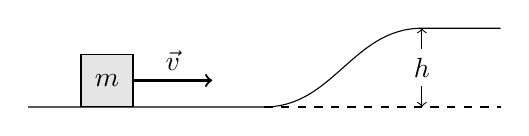
\begin{tikzpicture}
        %% Surface
        \draw (-3,0) -- (0,0) to [out=0,in=180] (2,1) -- (3,1);
        \draw[dashed] (0,0) -- (3,0);
        %% curve line
        \draw[<->] (2,0) -- (2,1) node[fill=white,anchor=center,pos=0.5] {$h$};
        %% Mass
        \node[draw,fill=white!90!black,minimum size=0.66cm,anchor=south] (M) at (-2,0) {$m$};
        \draw[thick,->] (M.east) -- ++(0:1) node[anchor=south,pos=0.5] {$\vec{v}$};
    \end{tikzpicture}
    \end{center}
    \begin{multicols}{3}
    \begin{choices}
        \wrongchoice{$gh$}
      \correctchoice{$mgh$}
        \wrongchoice{$\dfrac{gh}{2}$}
        \wrongchoice{$\dfrac{mgh}{2}$}
        \wrongchoice{$2mgh$}
    \end{choices}
    \end{multicols}
\end{question}
}

\element{halliday-mc}{
\begin{question}{halliday-ch08-q21}
    A \SI{2.2}{\kilo\gram} block starts from rest on a rough inclined plane that makes an angle of \ang{25} with the horizontal.
    The coefficient of kinetic friction is \num{0.25}.
    As the block goes \SI{2.0}{\meter} down the plane,
        the mechanical energy of the Earth-block system changes by:
    \begin{multicols}{3}
    \begin{choices}
        \wrongchoice{zero}
      \correctchoice{\SI{-9.8}{\joule}}
        \wrongchoice{\SI{9.8}{\joule}}
        \wrongchoice{\SI{-18}{\joule}}
        \wrongchoice{\SI{18}{\joule}}
    \end{choices}
    \end{multicols}
\end{question}
}

\element{halliday-mc}{
\begin{question}{halliday-ch08-q22}
    A simple pendulum consists of a \SI{2.0}{\kilo\gram} mass attached to a string.
    It is released from rest at $X$ as shown.
    \begin{center}
    \begin{tikzpicture}
        %% Ceiling
        \node[anchor=south,fill,pattern=north east lines,minimum width=4cm, minimum height=0.05cm] at (0,0) {};
        \draw (-2,0) -- (2,0);
        %% Pendulum
        \draw[thick] (0,0) -- (315:3); 
        \draw (225:3) arc (225:315:3);
        \draw[very thick,->] (315:3) arc (315:300:3);
        %% Labels
        \draw[fill] (270:3) circle (1pt) node[anchor=north] {$Y$};
        \draw[fill] (315:3) circle (5pt) node[anchor=south west] {$X$};
        \draw[dashed] (315:3) -- ++(0:1);
        \draw[dashed] (270:3) -- ++(0:3.1);
        \draw[thick,<-] (315:3) ++(0:0.9) --++(90:0.5);
        \path (315:3) ++(0:0.9) ++(270:0.44) node[anchor=center] {\SI{1.85}{\meter}};
        \draw[thick,<-] (270:3) ++(0:3.0) -- ++(270:0.5);
    \end{tikzpicture}
    \end{center}
    Its speed at the lowest point $Y$ is about:
    \begin{multicols}{2}
    \begin{choices}
        \wrongchoice{\SI{0.90}{\meter\per\second}}
        \wrongchoice{\SI[parse-numbers=false]{\sqrt{3.6}}{\meter\per\second}}
        \wrongchoice{\SI{3.6}{\meter\per\second}}
      \correctchoice{\SI{6.0}{\meter\per\second}}
        \wrongchoice{\SI{36}{\meter\per\second}}
    \end{choices}
    \end{multicols}
\end{question}
}

\element{halliday-mc}{
\begin{question}{halliday-ch08-q23}
    The long pendulum shown is drawn aside until the ball has risen \SI{0.50}{\meter}.
    \begin{center}
    \begin{tikzpicture}
        %% Ceiling
        \node[anchor=south,fill,pattern=north east lines,minimum width=4cm, minimum height=0.05cm] at (0,0) {};
        \draw (-2,0) -- (2,0);
        %% Pendulum
        \draw[thick] (0,0) -- (315:3); 
        \draw (225:3) arc (225:315:3);
        \draw[very thick,->] (315:3) arc (315:300:3);
        %% Labels
        \draw[fill] (315:3) circle (5pt);
        \draw[dashed] (315:3) -- ++(0:1);
        \draw[dashed] (270:3) -- ++(0:3.1);
        \draw[thick,<-] (315:3) ++(0:0.9) --++(90:0.5);
        \path (315:3) ++(0:0.9) ++(270:0.44) node[anchor=center] {\SI{0.5}{\meter}};
        \draw[thick,<-] (270:3) ++(0:3.0) -- ++(270:0.5);
    \end{tikzpicture}
    \end{center}
    It is then given an initial speed of \SI{3.0}{\meter\per\second}.
    The speed of the ball at its lowest position is:
    \begin{multicols}{3}
    \begin{choices}
        \wrongchoice{zero}
        \wrongchoice{\SI{0.89}{\meter\per\second}}
        \wrongchoice{\SI{3.1}{\meter\per\second}}
        \wrongchoice{\SI{3.7}{\meter\per\second}}
      \correctchoice{\SI{4.3}{\meter\per\second}}
    \end{choices}
    \end{multicols}
\end{question}
}

\element{halliday-mc}{
\begin{question}{halliday-ch08-q24}
    A particle moves along the $x$ axis under the influence of a stationary object.
    The net force on the particle is given by $F=\left(\SI{8}{\newton\per\meter\cubed}\right) x^3$.
    If the potential energy is taken to be zero for $x=0$ then the potential energy is given by:
    \begin{multicols}{2}
    \begin{choices}
        \wrongchoice{$\left(\SI{2}{\joule\per\meter\tothefourth}\right) x^4$}
      \correctchoice{$\left(\SI{-2}{\joule\per\meter\tothefourth}\right) x^4$}
        \wrongchoice{$\left(\SI{24}{\joule\per\meter\squared}\right) x^2$}
        \wrongchoice{$\left(\SI{-24}{\joule\per\meter\squared}\right) x^2$}
        \wrongchoice{$\SI{5}{\joule} - \left(\SI{2}{\joule\per\meter\tothefourth}\right) x^4$}
    \end{choices}
    \end{multicols}
\end{question}
}

\element{halliday-mc}{
\begin{question}{halliday-ch08-q25}
    A \SI{0.20}{\kilo\gram} particle moves along the $x$ axis under the influence of a stationary object.
    The potential energy is given by
    \begin{equation*}
        U\left(x\right) = \left(\SI{8.0}{\joule\per\meter\squared}\right) x^2 + \left(\SI{2.0}{\joule\per\meter\tothefourth}\right) x^4\, ,
    \end{equation*}
        where $x$ is in coordinate of the particle.
    If the particle has a speed of \SI{5.0}{\meter\per\second} when it is at $x=\SI{1.0}{\meter}$,
        its speed when it is at the origin is:
    \begin{multicols}{3}
    \begin{choices}
        \wrongchoice{zero}
        \wrongchoice{\SI{2.5}{\meter\per\second}}
        \wrongchoice{\SI{5.7}{\meter\per\second}}
        \wrongchoice{\SI{7.9}{\meter\per\second}}
      \correctchoice{\SI{11}{\meter\per\second}}
    \end{choices}
    \end{multicols}
\end{question}
}

\element{halliday-mc}{
\begin{question}{halliday-ch08-q26}
    Which of the five graphs correctly shows the potential energy of a spring as a function of its elongation?
    \begin{multicols}{2}
    \begin{choices}
        \AMCboxDimensions{down=-2.5em}
        \wrongchoice{
            \begin{tikzpicture}
                \begin{axis}[
                    axis y line=left,
                    axis x line=bottom,
                    axis line style={->},
                    xlabel={elongation},
                    xtick=\empty,
                    ylabel={energy},
                    ytick=\empty,
                    xmin=0,xmax=11,
                    ymin=0,ymax=11,
                    width=0.95\columnwidth,
                    very thin,
                ]
                \addplot[line width=1pt,domain=0:10]{8};
                \end{axis}
            \end{tikzpicture}
        }
        \wrongchoice{
            \begin{tikzpicture}
                \begin{axis}[
                    axis y line=left,
                    axis x line=bottom,
                    axis line style={->},
                    xlabel={elongation},
                    xtick=\empty,
                    ylabel={energy},
                    ytick=\empty,
                    xmin=0,xmax=11,
                    ymin=0,ymax=11,
                    width=0.95\columnwidth,
                    very thin,
                ]
                \addplot[line width=1pt,domain=0:10]{x};
                \end{axis}
            \end{tikzpicture}
        }
        %% ANS is C
        \correctchoice{
            \begin{tikzpicture}
                \begin{axis}[
                    axis y line=left,
                    axis x line=bottom,
                    axis line style={->},
                    xlabel={elongation},
                    xtick=\empty,
                    ylabel={energy},
                    ytick=\empty,
                    xmin=0,xmax=11,
                    ymin=0,ymax=11,
                    width=0.95\columnwidth,
                    very thin,
                ]
                \addplot[line width=1pt,domain=0:10]{0.1*x*x};
                \end{axis}
            \end{tikzpicture}
        }
        \wrongchoice{
            \begin{tikzpicture}
                \begin{axis}[
                    axis y line=left,
                    axis x line=bottom,
                    axis line style={->},
                    xlabel={elongation},
                    xtick=\empty,
                    ylabel={energy},
                    ytick=\empty,
                    xmin=0,xmax=11,
                    ymin=0,ymax=11,
                    width=0.95\columnwidth,
                    very thin,
                ]
                %% changed to sqrt
                \addplot[line width=1pt,domain=0:10]{3.1*sqrt(x)};
                \end{axis}
            \end{tikzpicture}
        }
        \wrongchoice{
            \begin{tikzpicture}
                \begin{axis}[
                    axis y line=left,
                    axis x line=bottom,
                    axis line style={->},
                    xlabel={elongation},
                    xtick=\empty,
                    ylabel={energy},
                    ytick=\empty,
                    xmin=0,xmax=11,
                    ymin=0,ymax=11,
                    width=0.95\columnwidth,
                    very thin,
                ]
                %% changed to inverse function
                \addplot[line width=1pt,domain=0:10]{10/x};
                \end{axis}
            \end{tikzpicture}
        }
    \end{choices}
    \end{multicols}
\end{question}
}

\element{halliday-mc}{
\begin{question}{halliday-ch08-q27}
    A force of \SI{10}{\newton} holds an ideal spring with a \SI{20}{\newton\per\meter} spring constant in compression.
    The potential energy stored in the spring is:
    \begin{multicols}{3}
    \begin{choices}
        \wrongchoice{\SI{0.5}{\joule}}
      \correctchoice{\SI{2.5}{\joule}}
        \wrongchoice{\SI{5}{\joule}}
        \wrongchoice{\SI{10}{\joule}}
        \wrongchoice{\SI{200}{\joule}}
    \end{choices}
    \end{multicols}
\end{question}
}

\element{halliday-mc}{
\begin{question}{halliday-ch08-q28}
    An ideal spring is used to fire a \SI{15.0}{\gram} pellet horizontally.
    The spring has a spring constant of \SI{20}{\newton\per\meter} and is initially compressed by 7.0 cm. The kinetic energy of the pellet as it leaves the spring is:
    \begin{multicols}{2}
    \begin{choices}
        \wrongchoice{zero}
        \wrongchoice{\SI{2.5e-2}{\joule}}
      \correctchoice{\SI{4.9e-2}{\joule}}
        \wrongchoice{\SI{9.8e-2}{\joule}}
        \wrongchoice{\SI{1.4}{\joule}}
    \end{choices}
    \end{multicols}
\end{question}
}

\element{halliday-mc}{
\begin{question}{halliday-ch08-q29}
    A \SI{0.50}{\kilo\gram} block attached to an ideal spring with a spring constant of \SI{80}{\newton\per\meter} oscillates on a horizontal frictionless surface.
    The total mechanical energy is \SI{0.12}{\joule}.
    The greatest extension of the spring from its equilibrium length is:
    \begin{multicols}{2}
    \begin{choices}
        \wrongchoice{\SI{1.5e-3}{\meter}}
        \wrongchoice{\SI{3.0e-3}{\meter}}
        \wrongchoice{\SI{0.039}{\meter}}
      \correctchoice{\SI{0.054}{\meter}}
        \wrongchoice{\SI{18}{\meter}}
    \end{choices}
    \end{multicols}
\end{question}
}

\element{halliday-mc}{
\begin{question}{halliday-ch08-q30}
    A \SI{0.50}{\kilo\gram} block attached to an ideal spring with a spring constant of \SI{80}{\newton\per\meter} oscillates on a horizontal frictionless surface.
    The total mechanical energy is \SI{0.12}{\joule}.
    The greatest speed of the block is:
    \begin{multicols}{3}
    \begin{choices}
        \wrongchoice{\SI{0.15}{\meter\per\second}}
        \wrongchoice{\SI{0.24}{\meter\per\second}}
        \wrongchoice{\SI{0.49}{\meter\per\second}}
      \correctchoice{\SI{0.69}{\meter\per\second}}
        \wrongchoice{\SI{1.46}{\meter\per\second}}
    \end{choices}
    \end{multicols}
\end{question}
}

\element{halliday-mc}{
\begin{question}{halliday-ch08-q31}
    A \SI{0.50}{\kilo\gram} block attached to an ideal spring with a spring constant of \SI{80}{\newton\per\meter} oscillates on a horizontal frictionless surface.
    When the spring is \SI{4.0}{\centi\meter} longer than its equilibrium length,
        the speed of the block is \SI{0.50}{\meter\per\second}.
    The greatest speed of the block is:
    \begin{multicols}{3}
    \begin{choices}
        \wrongchoice{\SI{0.23}{\meter\per\second}}
        \wrongchoice{\SI{0.32}{\meter\per\second}}
        \wrongchoice{\SI{0.55}{\meter\per\second}}
      \correctchoice{\SI{0.71}{\meter\per\second}}
        \wrongchoice{\SI{0.93}{\meter\per\second}}
    \end{choices}
    \end{multicols}
\end{question}
}

\element{halliday-mc}{
\begin{question}{halliday-ch08-q32}
    A \SI{0.5}{\kilo\gram} block slides along a horizontal frictionless surface at \SI{2}{\meter\per\second}.
    It is brought to rest by compressing a very long spring of spring constant \SI{800}{\newton\per\meter}.
    The maximum spring compression is:
    \begin{multicols}{3}
    \begin{choices}
        \wrongchoice{zero}
        \wrongchoice{\SI{3}{\centi\meter}}
      \correctchoice{\SI{5}{\centi\meter}}
        \wrongchoice{\SI{80}{\centi\meter}}
        \wrongchoice{\SI{80}{\centi\meter}}
    \end{choices}
    \end{multicols}
\end{question}
}

\element{halliday-mc}{
\begin{question}{halliday-ch08-q33}
    A block of mass $m$ is initially moving to the right on a horizontal frictionless surface at a speed $v$.
    It then compresses a spring of spring constant $k$.
    At the instant when the kinetic energy of the block is equal to the potential energy of the spring,
        the spring is compressed a distance of:
    \begin{multicols}{3}
    \begin{choices}
      \correctchoice{$v\sqrt{\dfrac{m}{2k}}$}
        \wrongchoice{$\dfrac{1}{2} mv^2$}
        \wrongchoice{$\dfrac{1}{4} mv^2$}
        \wrongchoice{$\dfrac{mv^2}{4k}$}
        \wrongchoice{$\dfrac{1}{4} \sqrt{\dfrac{mv}{k}}$}
    \end{choices}
    \end{multicols}
\end{question}
}

\element{halliday-mc}{
\begin{question}{halliday-ch08-q34}
    A \SI{700}{\newton} man jumps out of a window into a fire net \SI{10}{\meter} below.
    The net stretches \SI{2}{\meter} before bringing the man to rest and tossing him back into the air.
    The maximum potential energy of the net,
        compared to its unstretched potential energy, is:
    \begin{multicols}{3}
    \begin{choices}
        \wrongchoice{\SI{300}{\joule}}
        \wrongchoice{\SI{710}{\joule}}
        \wrongchoice{\SI{850}{\joule}}
        \wrongchoice{\SI{7000}{\joule}}
      \correctchoice{\SI{8400}{\joule}}
    \end{choices}
    \end{multicols}
\end{question}
}

%\element{halliday-mc}{
%\begin{question}{halliday-ch08-q35}
%    A toy cork gun contains a spring whose spring constant is \SI{10.0}{\newton\per\meter}.
%    The spring is compressed \SI{5.00}{\centi\meter} and then used to propel a \SI{6.00}{\gram} cork.
%    The cork, however,
%        sticks to the spring for \SI{1.00}{\centi\meter} beyond its unstretched length before separation occurs.
%    \begin{center}
%    \begin{tikzpicture}
%        %% NOTE:
%    \end{tikzpicture}
%    \end{center}
%    The muzzle velocity of this cork is:
%    \begin{multicols}{3}
%    \begin{choices}
%        \wrongchoice{\SI{1.02}{\meter\per\second}}
%        \wrongchoice{\SI{1.41}{\meter\per\second}}
%      \correctchoice{\SI{2.00}{\meter\per\second}}
%        \wrongchoice{\SI{2.04}{\meter\per\second}}
%        \wrongchoice{\SI{4.00}{\meter\per\second}}
%    \end{choices}
%    \end{multicols}
%\end{question}
%}

\element{halliday-mc}{
\begin{question}{halliday-ch08-q36}
    A small object of mass $m$, on the end of a light cord,
        is held horizontally at a distance $r$ from a fixed support as shown.
    \begin{center}
    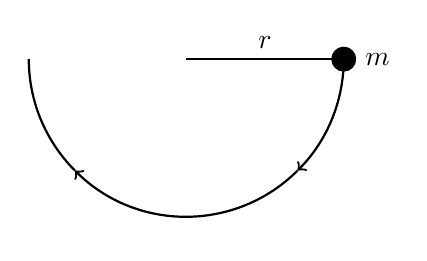
\begin{tikzpicture}
        \draw[thick] (0,0) -- (2,0) node[pos=0.5,anchor=south] {$r$};
        \draw[fill] (2,0) circle (1.0ex) node[xshift=1ex,anchor=west] {$m$};
        \draw[thick,->] (360:2) arc(360:315:2);
        \draw[thick,->] (315:2) arc(315:225:2);
        \draw[thick] (225:2) arc(225:180:2);
    \end{tikzpicture}
    \end{center}
    The object is then released.
    What is the tension force of the cord when the object is at the lowest point of its swing?
    \begin{multicols}{3}
    \begin{choices}
        \wrongchoice{$\dfrac{mg}{2}$}
        \wrongchoice{$mg$}
        \wrongchoice{$2mg$}
      \correctchoice{$3mg$}
        \wrongchoice{$mgr$}
    \end{choices}
    \end{multicols}
\end{question}
}

\element{halliday-mc}{
\begin{question}{halliday-ch08-q37}
    The string in the figure is \SI{50}{\centi\meter} long.
    \begin{center}
    \begin{tikzpicture}
        \draw[thick] (0,0) -- (2,0) node[pos=0.5,anchor=south] {\SI{50}{\centi\meter}};
        \draw[fill] (2,0) circle (1.0ex) node[xshift=1ex,anchor=west] {$m$};
        \draw[dashed,thick,->] (360:2) arc(360:315:2);
        \draw[dashed,thick,->] (315:2) arc(315:225:2);
        \draw[dashed,thick] (225:2) arc(225:180:2);
    \end{tikzpicture}
    \end{center}
    When the ball is released from rest,
        it swings along the dotted arc.
    How fast is it going at the lowest point in its swing?
    \begin{multicols}{3}
    \begin{choices}
        \wrongchoice{\SI{2.0}{\meter\per\second}}
        \wrongchoice{\SI{2.2}{\meter\per\second}}
      \correctchoice{\SI{3.1}{\meter\per\second}}
        \wrongchoice{\SI{4.4}{\meter\per\second}}
        \wrongchoice{\SI{6.0}{\meter\per\second}}
    \end{choices}
    \end{multicols}
\end{question}
}

\element{halliday-mc}{
\begin{question}{halliday-ch08-q38}
    A block is released from rest at point $P$ and slides along the frictionless track shown.
    \begin{center}
    \begin{tikzpicture}
        %% Ground
        \draw (-1,0) -- (5,0);
        \node[anchor=north,fill,pattern=north east lines,minimum width=6cm, minimum height=0.05cm] at (2,0) {};
        %% Path
        \draw[thick] (-1,3) -- (0,3) to[out=0,in=180] (2,0.5) to[out=0,in=180] (4,1.25) to [out=0,in=135] (5,0.25);
        %% Mass
        \draw[thick] node[draw,fill=white!90!black,minimum size=0.5cm,anchor=south] (M) at (0,3) {$m$};
        %% Labels
        \node[anchor=south east] at (-0.5,3) {$P$};
        \node[anchor=south] at (4,1.25) {$Q$};
        \draw[<->] (0,0) -- (0,3) node[pos=0.5,fill=white,anchor=center] {$h_1$};
        \draw[<->] (4,0) -- (4,1.25) node[pos=0.5,fill=white,anchor=center] {$h_2$};
    \end{tikzpicture}
    \end{center}
    At point $Q$, its speed is:
    \begin{multicols}{2}
    \begin{choices}
        \wrongchoice{$2g\sqrt{h_1-h_2}$}
        \wrongchoice{$2g\left(h_1-h_2\right)$}
        \wrongchoice{$\dfrac{h_1-h_2}{2g}$}
      \correctchoice{$\sqrt{2g\left(h_1-h_2\right)}$}
        \wrongchoice{$\dfrac{\left(h_1-h_2\right)^2}{2g}$}
    \end{choices}
    \end{multicols}
\end{question}
}

\element{halliday-mc}{
\begin{question}{halliday-ch08-q39}
    A small object of mass $m$ starts from rest at the position shown and slides along the frictionless loop-the-loop track of radius $R$.
    \begin{center}
    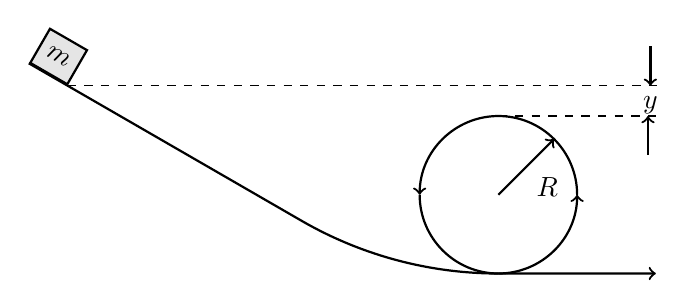
\begin{tikzpicture}
        %% Track
        \draw[thick] (0,0) arc(270:240:5) -- ++(150:4) node[draw,fill=white!90!black,minimum size=0.5cm,anchor=south west,rotate=-30] (M) {$m$};
        \draw[thick,->] (0,0) arc (270:360:1);
        \draw[thick,->] (1,1) arc (0:180:1);
        \draw[thick,->] (-1,1) arc (180:270:1) -- ++(0:2);
        \draw[thick,->] (0,1) -- ++(45:1) node[pos=0.5,anchor=north west] {$R$};
        %% Labels
        \draw[dashed] (M.south east) -- ++(0:7.5);
        \draw[thick,<-] (M.south east) ++(0:7.4) -- ++(90:0.5);
        \path (M.south east) ++(0:7.4) ++(270:0.25) node[anchor=center] {$y$};
        \draw[dashed] (0,2) -- ++(0:2);
        \draw[thick,<-] (0,2) ++(0:1.9) --++(270:0.5);
    \end{tikzpicture}
    \end{center}
    What is the smallest value of $y$ such that the object will slide without losing contact with the track?
    \begin{multicols}{3}
    \begin{choices}
        \wrongchoice{$\dfrac{R}{4}$}
      \correctchoice{$\dfrac{R}{2}$}
        \wrongchoice{$R$}
        \wrongchoice{$2R$}
        \wrongchoice{zero}
    \end{choices}
    \end{multicols}
\end{question}
}

\element{halliday-mc}{
\begin{question}{halliday-ch08-q40}
    A small object slides along the frictionless loop-the-loop with a diameter of \SI{3}{\meter}.
    \begin{center}
    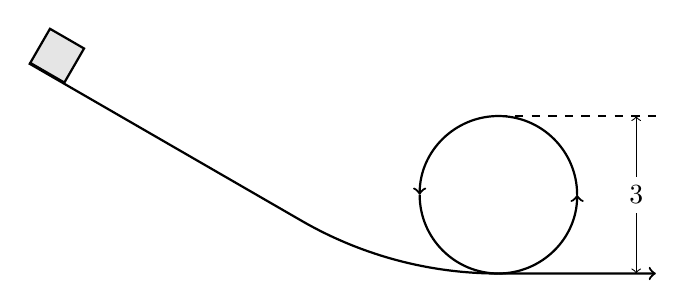
\begin{tikzpicture}
        %% Track
        \draw[thick] (0,0) arc(270:240:5) -- ++(150:4) node[draw,fill=white!90!black,minimum size=0.5cm,anchor=south west,rotate=-30] (M) {};
        \draw[thick,->] (0,0) arc (270:360:1);
        \draw[thick,->] (1,1) arc (0:180:1);
        \draw[thick,->] (-1,1) arc (180:270:1) -- ++(0:2);
        %% Labels
        \draw[dashed] (0,2) -- ++(0:2);
        \draw[<->] (1.75,0) -- ++(90:2) node[pos=0.5,anchor=center,fill=white] {\SI{3}{\meter}};
    \end{tikzpicture}
    \end{center}
    What minimum speed must it have at the top of the loop?
    \begin{multicols}{3}
    \begin{choices}
        \wrongchoice{\SI{1.9}{\meter\per\second}}
      \correctchoice{\SI{3.8}{\meter\per\second}}
        \wrongchoice{\SI{5.4}{\meter\per\second}}
        \wrongchoice{\SI{15}{\meter\per\second}}
        \wrongchoice{\SI{29}{\meter\per\second}}
    \end{choices}
    \end{multicols}
\end{question}
}

\element{halliday-mc}{
\begin{question}{halliday-ch08-q41}
    A rectangular block is moving along a frictionless path when it encounters the circular loop as shown.
    \begin{center}
    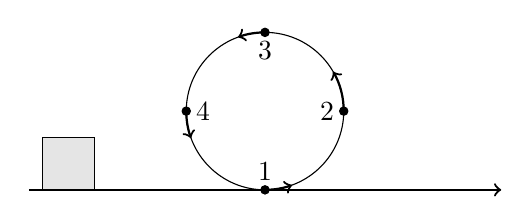
\begin{tikzpicture}
        %% Track
        \draw[thick,->] (-3,0) -- (3,0);
        \draw (0,1) circle (1cm);
        \draw[thick,->] (0,0) arc (270:290:1);
        \draw[thick,->] (1,1) arc (0:30:1);
        \draw[thick,->] (0,2) arc (90:110:1);
        \draw[thick,->] (-1,1) arc (180:200:1);
        %% Marks
        \draw[fill] (0,0) circle (1.5pt) node[anchor=south] {1};
        \draw[fill] (1,1) circle (1.5pt) node[anchor=east] {2};
        \draw[fill] (0,2) circle (1.5pt) node[anchor=north] {3};
        \draw[fill] (-1,1) circle (1.5pt) node[anchor=west] {4};
        %% Block
        \node[draw,fill=white!90!black,minimum size=0.66cm,anchor=south] (M) at (-2.5,0) {};
    \end{tikzpicture}
    \end{center}
    The block passes points 1, 2, 3, 4, 1 before returning to the horizontal track.
    At point 3:
    \begin{choices}
        \wrongchoice{its mechanical energy is a minimum}
        \wrongchoice{the forces on it are balanced}
        \wrongchoice{it is not accelerating}
      \correctchoice{its speed is a minimum}
        \wrongchoice{it experiences a net upward force}
    \end{choices}
\end{question}
}

\element{halliday-mc}{
\begin{question}{halliday-ch08-q42}
    A ball of mass $m$, at one end of a string of length $L$,
        rotates in a vertical circle just fast enough to prevent the string from going slack at the top of the circle.
    \begin{center}
    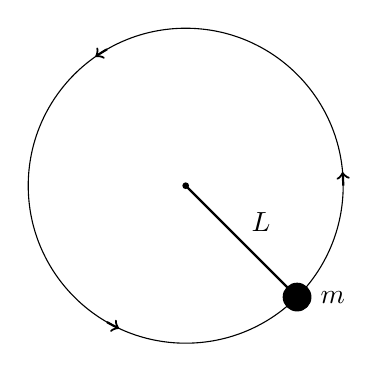
\begin{tikzpicture}
        %% Path
        \draw (0,0) circle (2cm);
        \draw[thick,->] (0:2) arc(0:5:2);
        \draw[thick,->] (120:2) arc(120:125:2);
        \draw[thick,->] (240:2) arc(240:245:2);
        %% Mass on string
        \draw[fill] (0,0) circle (1pt);
        \draw[fill] (315:2) circle (5pt) node[anchor=west,xshift=5pt] {$m$};
        \draw[thick,->] (0,0) -- (315:2) node[pos=0.5,anchor=south west] {$L$};
    \end{tikzpicture}
    \end{center}
    The speed of the ball at the bottom of the circle is:
    \begin{multicols}{3}
    \begin{choices}
        \wrongchoice{$\sqrt{2gL}$}
        \wrongchoice{$\sqrt{3gL}$}
        \wrongchoice{$\sqrt{4gL}$}
      \correctchoice{$\sqrt{5gL}$}
        \wrongchoice{$\sqrt{7gL}$}
    \end{choices}
    \end{multicols}
\end{question}
}

%\element{halliday-mc}{
%\begin{question}{halliday-ch08-q43}
%    A particle is released from rest at the point $x=a$ and moves along the $x$ axis subject to the potential energy function $U(x)$ shown.
%    \begin{center}
%    \begin{tikzpicture}
%        %% NOTE:
%    \end{tikzpicture}
%    \end{center}
%    The particle:
%    \begin{choices}
%        \wrongchoice{moves to a point to the left of $x=e$, stops, and remains at rest}
%      \correctchoice{moves to a point to $x=e$, then moves to the left}
%        \wrongchoice{moves to infinity at varying speed}
%        \wrongchoice{moves to $x=b$, where it remains at rest}
%        \wrongchoice{moves to $x=e$ and then to $x=d$, where it remains at rest}
%    \end{choices}
%\end{question}
%}

\element{halliday-mc}{
\begin{question}{halliday-ch08-q44}
    The potential energy of a particle moving along the $x$ axis is given by
    \begin{equation*}
        U\left(x\right) = \left(\SI{8.0}{\joule\per\meter\squared}\right) x^2 + \left(\SI{2.0}{\joule\per\meter\tothefourth}\right) x^4 .
    \end{equation*}
    If the total mechanical energy is \SI{9.0}{\joule},
        the limits of motion are:
    \begin{multicols}{2}
    \begin{choices}
      \correctchoice{\SI{-0.96}{\meter};    \SI{+0.96}{\meter}}
        \wrongchoice{\SI{-2.2}{\meter};     \SI{+2.2}{\meter}}
        \wrongchoice{\SI{-1.6}{\meter};     \SI{+1.6}{\meter}}
        \wrongchoice{\SI{-0.96}{\meter};    \SI{+2.2}{\meter}}
        \wrongchoice{\SI{-0.96}{\meter};    \SI{+1.6}{\meter}}
    \end{choices}
    \end{multicols}
\end{question}
}

\element{halliday-mc}{
\begin{question}{halliday-ch08-q45}
    The potential energy of a \SI{0.20}{\kilo\gram} particle moving along the $x$ axis is given by
    \begin{equation*}
        U\left(x\right) = \left(\SI{8.0}{\joule\per\meter\squared}\right) x^2 + \left(\SI{2.0}{\joule\per\meter\tothefourth}\right) x^4 .
    \end{equation*}
    When the particle is at $x=\SI{1.0}{\meter}$ it is traveling in the positive $x$ direction with a speed of \SI{5.0}{\meter\per\second}.
    It next stops momentarily to turn around at $x= $
    \begin{multicols}{3}
    \begin{choices}
        \wrongchoice{zero}
        \wrongchoice{\SI{-1.1}{\meter}}
      \correctchoice{\SI{1.1}{\meter}}
        \wrongchoice{\SI{-2.3}{\meter}}
        \wrongchoice{\SI{2.3}{\meter}}
    \end{choices}
    \end{multicols}
\end{question}
}

\element{halliday-mc}{
\begin{question}{halliday-ch08-q46}
    Given a potential energy function $U\left(x\right)$,
        the corresponding force $\vec{F}$ is in the positive $x$ direction if:
    \begin{choices}
        \wrongchoice{$U$ is positive}
        \wrongchoice{$U$ is negative}
        \wrongchoice{$U$ is an increasing function of $x$}
      \correctchoice{$U$ is a decreasing function of $x$}
        \wrongchoice{it is impossible to obtain the direction of $\vec{F}$ from $U$}
    \end{choices}
\end{question}
}

\element{halliday-mc}{
\begin{question}{halliday-ch08-q47}
    As a particle moves along the $x$ axis it is acted upon by a conservative force.
    The potential energy is shown below as a function of the coordinate $x$ of the particle.
    \begin{center}
    \begin{tikzpicture}
        \begin{axis}[
            axis y line=left,
            axis x line=middle,
            axis line style={->},
            xlabel={$x$},
            x label style={
                at={(current axis.right of origin)},
                anchor=west,
            },
            xtick={2,4,6,7},
            xticklabels={$A$,$B$,$C$,$D$},
            ylabel={$U(x)$},
            y label style={
                at={(current axis.above origin)},
                anchor=south,
                rotate=270,
            },
            ytick=\empty,
            grid=major,
            xmin=0,xmax=8,
            ymin=0,ymax=10,
            width=0.8\columnwidth,
            height=0.5\columnwidth,
            very thin,
        ]
        \addplot[line width=1pt,mark=\empty] coordinates { (0,7) (2,7) (4,2) (6,2) (7,10)};
        \end{axis}
    \end{tikzpicture}
    \end{center}
    Rank the labeled regions according to the magnitude of the force,
        least to greatest.
    \begin{multicols}{2}
    \begin{choices}
        \wrongchoice{AB, BC, CD}
        \wrongchoice{AB, CD, BC}
        \wrongchoice{BC, CD, AB}
      \correctchoice{BC, AB, CD}
        \wrongchoice{CD, BC, AB}
    \end{choices}
    \end{multicols}
\end{question}
}

\element{halliday-mc}{
\begin{question}{halliday-ch08-q48}
    The first graph shows the potential energy $U (x)$ for a particle moving on the $x$ axis.
    \begin{center}
    \begin{tikzpicture}
        \begin{axis}[
            axis y line=middle,
            axis x line=middle,
            axis line style={->},
            xlabel={$x$},
            x label style={
                at={(current axis.right of origin)},
                anchor=west,
            },
            xtick=\empty,
            ylabel={$U$},
            y label style={
                at={(current axis.above origin)},
                anchor=south,
            },
            ytick=\empty,
            xmin=0,xmax=11,
            ymin=0,ymax=11,
            width=0.8\columnwidth,
            height=0.5\columnwidth,
            very thin,
        ]
        \addplot[line width=1pt,domain=0:10]{0.4*(x-5)*(x-5)};
        \end{axis}
    \end{tikzpicture}
    \end{center}
    Which of the other five graphs correctly gives the force $F$ exerted on the particle?
    \begin{multicols}{2}
    \begin{choices}
        %% ANS is D
        \AMCboxDimensions{down=-2.5em}
        \wrongchoice{
            \begin{tikzpicture}
                \begin{axis}[
                    axis y line=middle,
                    axis x line=middle,
                    axis line style={->},
                    xlabel={$x$},
                    x label style={
                        at={(current axis.right of origin)},
                        anchor=west,
                    },
                    xtick=\empty,
                    ylabel={$F$},
                    y label style={
                        at={(current axis.above origin)},
                        anchor=south,
                    },
                    ytick=\empty,
                    xmin=0,xmax=10,
                    ymin=-10,ymax=11,
                    width=0.95\columnwidth,
                    very thin,
                ]
                \addplot[line width=1pt,domain=0:10]{0.08*(x-5)*(x-5)*(x-5)};
                \end{axis}
            \end{tikzpicture}
        }
        \wrongchoice{
            \begin{tikzpicture}
                \begin{axis}[
                    axis y line=middle,
                    axis x line=middle,
                    axis line style={->},
                    xlabel={$x$},
                    x label style={
                        at={(current axis.right of origin)},
                        anchor=west,
                    },
                    xtick=\empty,
                    ylabel={$F$},
                    y label style={
                        at={(current axis.above origin)},
                        anchor=south,
                    },
                    ytick=\empty,
                    xmin=0,xmax=10,
                    ymin=-10,ymax=11,
                    width=0.95\columnwidth,
                    very thin,
                ]
                \addplot[line width=1pt,domain=0:10]{-0.4*(x-5)*(x-5)};
                \end{axis}
            \end{tikzpicture}
        }
        \wrongchoice{
            \begin{tikzpicture}
                \begin{axis}[
                    axis y line=middle,
                    axis x line=middle,
                    axis line style={->},
                    xlabel={$x$},
                    x label style={
                        at={(current axis.right of origin)},
                        anchor=west,
                    },
                    xtick=\empty,
                    ylabel={$F$},
                    y label style={
                        at={(current axis.above origin)},
                        anchor=south,
                    },
                    ytick=\empty,
                    xmin=-10,xmax=10,
                    ymin=-10,ymax=11,
                    width=0.95\columnwidth,
                    very thin,
                ]
                \addplot[line width=1pt,domain=-10:10]{-x};
                \end{axis}
            \end{tikzpicture}
        }
        %% ANS is D
        \correctchoice{
            \begin{tikzpicture}
                \begin{axis}[
                    axis y line=middle,
                    axis x line=middle,
                    axis line style={->},
                    xlabel={$x$},
                    x label style={
                        at={(current axis.right of origin)},
                        anchor=west,
                    },
                    xtick=\empty,
                    ylabel={$F$},
                    y label style={
                        at={(current axis.above origin)},
                        anchor=south,
                    },
                    ytick=\empty,
                    xmin=0,xmax=10,
                    ymin=-10,ymax=11,
                    width=0.95\columnwidth,
                    very thin,
                ]
                \addplot[line width=1pt,domain=0:10]{10-2*x};
                \end{axis}
            \end{tikzpicture}
        }
        \wrongchoice{
            \begin{tikzpicture}
                \begin{axis}[
                    axis y line=middle,
                    axis x line=middle,
                    axis line style={->},
                    xlabel={$x$},
                    x label style={
                        at={(current axis.right of origin)},
                        anchor=west,
                    },
                    xtick=\empty,
                    ylabel={$F$},
                    y label style={
                        at={(current axis.above origin)},
                        anchor=south,
                    },
                    ytick=\empty,
                    xmin=0,xmax=10,
                    ymin=-10,ymax=11,
                    width=0.95\columnwidth,
                    very thin,
                ]
                \addplot[line width=1pt,domain=0:10]{0.4*(x-5)*(x-5)};
                \end{axis}
            \end{tikzpicture}
        }
        %% Added for symmetry
        \wrongchoice{
            \begin{tikzpicture}
                \begin{axis}[
                    axis y line=middle,
                    axis x line=middle,
                    axis line style={->},
                    xlabel={$x$},
                    x label style={
                        at={(current axis.right of origin)},
                        anchor=west,
                    },
                    xtick=\empty,
                    ylabel={$F$},
                    y label style={
                        at={(current axis.above origin)},
                        anchor=south,
                    },
                    ytick=\empty,
                    xmin=-10,xmax=10,
                    ymin=-10,ymax=11,
                    width=0.95\columnwidth,
                    very thin,
                ]
                \addplot[line width=1pt,domain=-10:10]{x};
                \end{axis}
            \end{tikzpicture}
        }
    \end{choices}
    \end{multicols}
\end{question}
}

%\newcommand{\hallidayChEightQFortyNine}{
%\begin{tikzpicture}
%    %% NOTE:
%\end{tikzpicture}
%}
%
%\element{halliday-mc}{
%\begin{question}{halliday-ch08-q49}
%    The diagram shows a plot of the potential energy as a function of $x$ for a particle moving along the $x$ axis.
%    \begin{center}
%        \hallidayChEightQFortyNine
%    \end{center}
%    The points of stable equilibrium are:
%    \begin{multicols}{3}
%    \begin{choices}
%        \wrongchoice{only $a$}
%      \correctchoice{only $b$}
%        \wrongchoice{only $c$}
%        \wrongchoice{only $d$}
%        \wrongchoice{$b$ and $d$}
%    \end{choices}
%    \end{multicols}
%\end{question}
%}
%
%\element{halliday-mc}{
%\begin{question}{halliday-ch08-q50}
%    The diagram shows a plot of the potential energy as a function of $x$ for a particle moving along the $x$ axis.
%    \begin{center}
%        \hallidayChEightQFortyNine
%    \end{center}
%    The points of unstable equilibrium are:
%    \begin{multicols}{3}
%    \begin{choices}
%        \wrongchoice{only $a$}
%        \wrongchoice{only $b$}
%        \wrongchoice{only $c$}
%      \correctchoice{only $d$}
%        \wrongchoice{$b$ and $d$}
%    \end{choices}
%    \end{multicols}
%\end{question}
%}

%\element{halliday-mc}{
%\begin{question}{halliday-ch08-q51}
%    The diagram shows a plot of the potential energy as a function of $x$ for a particle moving along the $x$ axis.
%    \begin{center}
%        \hallidayChEightQFortyNine
%    \end{center}
%    Of the labeled points, the points of neutral equilibrium are:
%    \begin{multicols}{3}
%    \begin{choices}
%        \wrongchoice{only $a$}
%        \wrongchoice{only $b$}
%      \correctchoice{only $c$}
%        \wrongchoice{only $d$}
%        \wrongchoice{$b$ and $d$}
%    \end{choices}
%    \end{multicols}
%\end{question}
%}

\element{halliday-mc}{
\begin{question}{halliday-ch08-q52}
    The potential energy of a body of mass $m$ is given by $U = -mgx + \dfrac{1}{2} kx^2$.
    The corresponding force is:
    \begin{multicols}{2}
    \begin{choices}
        \wrongchoice{$-\dfrac{mgx^2}{2} + \dfrac{kx^3}{6}$}
        \wrongchoice{$\dfrac{mgx^2}{2} - \dfrac{kx^3}{6}$}
        \wrongchoice{$-mg + \dfrac{kx}{2}$}
        \wrongchoice{$-mg + kx$}
      \correctchoice{$mg - kx$}
    \end{choices}
    \end{multicols}
\end{question}
}

\element{halliday-mc}{
\begin{question}{halliday-ch08-q53}
    The potential energy of a \SI{0.20}{\kilo\gram} particle moving along the $x$ axis is given by
    \begin{equation*}
        U\left(x\right) = \left(\SI{8.0}{\joule\per\meter\squared}\right) x^2 + \left(\SI{2.0}{\joule\per\meter\tothefourth}\right) x^4\, .
    \end{equation*}
    When the particle is at $x=\SI{1.0}{\meter}$ the magnitude of its acceleration is:
    \begin{multicols}{3}
    \begin{choices}
        \wrongchoice{zero}
        %% NOTE: Were +/- 8 and +/- 40
        \wrongchoice{\SI{-40}{\meter\per\second\squared}}
        \wrongchoice{\SI{40}{\meter\per\second\squared}}
      \correctchoice{\SI{-120}{\meter\per\second\squared}}
        \wrongchoice{\SI{120}{\meter\per\second\squared}}
    \end{choices}
    \end{multicols}
\end{question}
}

\element{halliday-mc}{
\begin{question}{halliday-ch08-q54}
    The potential energy for the interaction between the two atoms in a diatomic molecule is $U = A x^{-12} - B x^{-6}$,
        where $A$ and $B$ are constants
    \begin{center}
    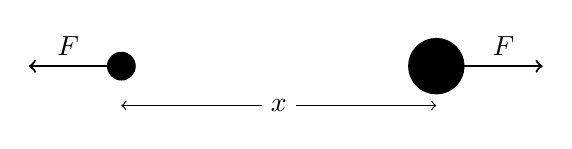
\begin{tikzpicture}
        %% Balls
        \draw[fill] (-2,0) circle (5pt);
        \draw[fill] (+2,0) circle (10pt);
        %% Vectors
        \draw[thick,->] (-2,0) ++(-5pt,0)  -- ++(180:1) node[pos=0.5,anchor=south] {$F$};
        \draw[thick,->] (+2,0) ++(10pt,0) -- ++(0:1) node[pos=0.5,anchor=south] {$F$};
        %% Distance
        \draw[<->] (-2,-0.5) -- (+2,-0.5) node[pos=0.5,anchor=center,fill=white] {$x$};
    \end{tikzpicture}
    \end{center}
    The magnitude of the force of one atom on the other is:
    \begin{choices}
      \correctchoice{$12 A \left|x\right|^{-13} - 6 B \left|x\right|^{-7}$}
        \wrongchoice{$-13 A \left|x\right|^{-13} + 7 B \left|x\right|^{-7}$}
        \wrongchoice{$-11 A \left|x\right|^{-11} + 5 B \left|x\right|^{-5}$}
        \wrongchoice{$72 A \left|x\right|^{-12} - 72 B \left|x\right|^{-6}$}
        \wrongchoice{$A \left|x\right|^{-13} - B \left|x\right|^{-7}$}
    \end{choices}
\end{question}
}

\element{halliday-mc}{
\begin{question}{halliday-ch08-q55}
    The thermal energy of a system consisting of a thrown ball,
        Earth, and the air is most closely associated with:
    \begin{choices}
        \wrongchoice{the gravitational interaction of Earth and the ball}
        \wrongchoice{the kinetic energy of the ball as a whole}
        \wrongchoice{motions of the individual particles within the ball}
      \correctchoice{motions of individual particles within the ball and the air}
        \wrongchoice{the kinetic energy of Earth as a whole}
    \end{choices}
\end{question}
}

\element{halliday-mc}{
\begin{question}{halliday-ch08-q56}
    Three identical blocks move either on a horizontal surface,
        up a plane, or down a plane, as shown below.
    They start with different speeds and continue to move until brought to rest by friction.
    They all move the same distance.
    \begin{center}
    \hfill
    \begin{tikzpicture}
        %% Ground
        \node[anchor=north,fill,pattern=north east lines,minimum width=2cm, minimum height=0.05cm] at (0,0) {};
        \draw (-1,0) -- (1,0);
        \node[anchor=north,yshift=-0.50cm] at (0,0) {$1$};
        %% Mass
        \node[draw,fill=white!90!black,minimum size=0.75cm,anchor=south] (M) at (0,0) {};
        %% Vectors
        \draw[thick,->] (M.east) -- ++(0:1cm) node[anchor=south,pos=0.5] {$\vec{v}$};
    \end{tikzpicture}
    \hfill
    \begin{tikzpicture}
        %% Ground
        \node[anchor=north,fill,pattern=horizontal lines,minimum width=2cm, minimum height=0.05cm,rotate=45] at (0,0) {};
        \draw (225:1) -- (45:1);
        \node[anchor=north,yshift=-0.50cm] at (0,0) {$2$};
        %% Mass
        \node[draw,fill=white!90!black,minimum size=0.75cm,anchor=south,rotate=45] (M) at (0,0) {};
        %% Vectors
        \draw[thick,->] (M.east) -- ++(45:1cm) node[anchor=south east,pos=0.8] {$\vec{v}$};
    \end{tikzpicture}
    \hfill
    \begin{tikzpicture}
        %% Ground
        \node[anchor=north,fill,pattern=horizontal lines,minimum width=2cm, minimum height=0.05cm,rotate=45] at (0,0) {};
        \draw (225:1) -- (45:1);
        \node[anchor=north,yshift=-0.50cm] at (0,0) {$3$};
        %% Mass
        \node[draw,fill=white!90!black,minimum size=0.75cm,anchor=south,rotate=45] (M) at (0,0) {};
        %% Vectors
        \draw[thick,->] (M.west) -- ++(225:1cm) node[anchor=south east,pos=0.8] {$\vec{v}$};
    \end{tikzpicture}
    \hfill
    \end{center}
    Rank the three situations according to the initial speeds,
        least to greatest.
    \begin{choices}
        \wrongchoice{The same for all cases}
        \wrongchoice{1, 2, 3}
        \wrongchoice{1, then 2 and 3 tie}
      \correctchoice{3, 1, 2}
        \wrongchoice{2, 1, 3}
    \end{choices}
\end{question}
}

\element{halliday-mc}{
\begin{question}{halliday-ch08-q57}
    Objects $A$ and $B$ interact with each other via both conservative and nonconservative forces.
    Let $K_A$ and $K_B$ be the kinetic energies,
        $U$ be the potential energy,
        and $E_{int}$ be the thermal energy.
    If no external agent does work on the objects then:
    \begin{choices}
        \wrongchoice{$K_A + U$ is conserved}
        \wrongchoice{$K_A + U + E_{int}$ is conserved}
        \wrongchoice{$K_A + K_B + E_{int}$ is conserved}
        \wrongchoice{$K_A + K_B + U$ is conserved}
      \correctchoice{$K_A + K_B + U + E_{int}$ is conserved}
    \end{choices}
\end{question}
}

\element{halliday-mc}{
\begin{question}{halliday-ch08-q58}
    A block slides across a rough horizontal table top.
    The work done by friction changes:
    \begin{choices}
        \wrongchoice{only the kinetic energy}
        \wrongchoice{only the potential energy}
        \wrongchoice{only the internal energy}
        \wrongchoice{only the kinetic and potential energies}
      \correctchoice{only the kinetic and internal energies}
    \end{choices}
\end{question}
}

\element{halliday-mc}{
\begin{question}{halliday-ch08-q59}
    A \SI{25}{\gram} ball is released from rest \SI{80}{\meter} above the surface of Earth.
    During the fall the total internal energy of the ball and air increases by \SI{15}{\joule}.
    Just before it hits the surface its speed is:
    \begin{multicols}{3}
    \begin{choices}
      \correctchoice{\SI{19}{\meter\per\second}}
        \wrongchoice{\SI{36}{\meter\per\second}}
        \wrongchoice{\SI{40}{\meter\per\second}}
        \wrongchoice{\SI{45}{\meter\per\second}}
        \wrongchoice{\SI{53}{\meter\per\second}}
    \end{choices}
    \end{multicols}
\end{question}
}

\element{halliday-mc}{
\begin{question}{halliday-ch08-q60}
    A \SI{5}{\kilo\gram} projectile is fired over level ground with a velocity of \SI{200}{\meter\per\second} at an angle of \ang{25} above the horizontal.
    Just before it hits the ground its speed is \SI{150}{\meter\per\second}.
    Over the entire trip the change in the internal energy of the projectile and air is:
    \begin{multicols}{2}
    \begin{choices}
        \wrongchoice{\SI{+19 000}{\joule}}
        \wrongchoice{\SI{-19 000}{\joule}}
      \correctchoice{\SI{+44 000}{\joule}}
        \wrongchoice{\SI{-44 000}{\joule}}
        \wrongchoice{zero}
    \end{choices}
    \end{multicols}
\end{question}
}

\element{halliday-mc}{
\begin{question}{halliday-ch08-q61}
    A \SI{0.75}{\kilo\gram} block slides on a rough horizontal table top.
    Just before it hits a horizontal ideal spring its speed is \SI{3.5}{\meter\per\second}.
    It compresses the spring \SI{5.7}{\centi\meter} before coming to rest.
    If the spring constant is \SI{1200}{\newton\per\meter},
        the internal energy of the block and the table top must have:
    \begin{multicols}{2}
    \begin{choices}
        \wrongchoice{not changed}
        \wrongchoice{decreased by \SI{1.9}{\joule}}
      \correctchoice{decreased by \SI{2.6}{\joule}}
        \wrongchoice{increased by \SI{1.9}{\joule}}
        \wrongchoice{increased by \SI{2.6}{\joule}}
    \end{choices}
    \end{multicols}
\end{question}
}


\endinput


